\chapter{Experimente}
\label{ch:experimente}

\section{Objekterkennung}
\subsection{Vortrainiertes Modell auf DocBank}
\begin{figure}[H]
    \centering
    \captionsetup{width=1\linewidth}
    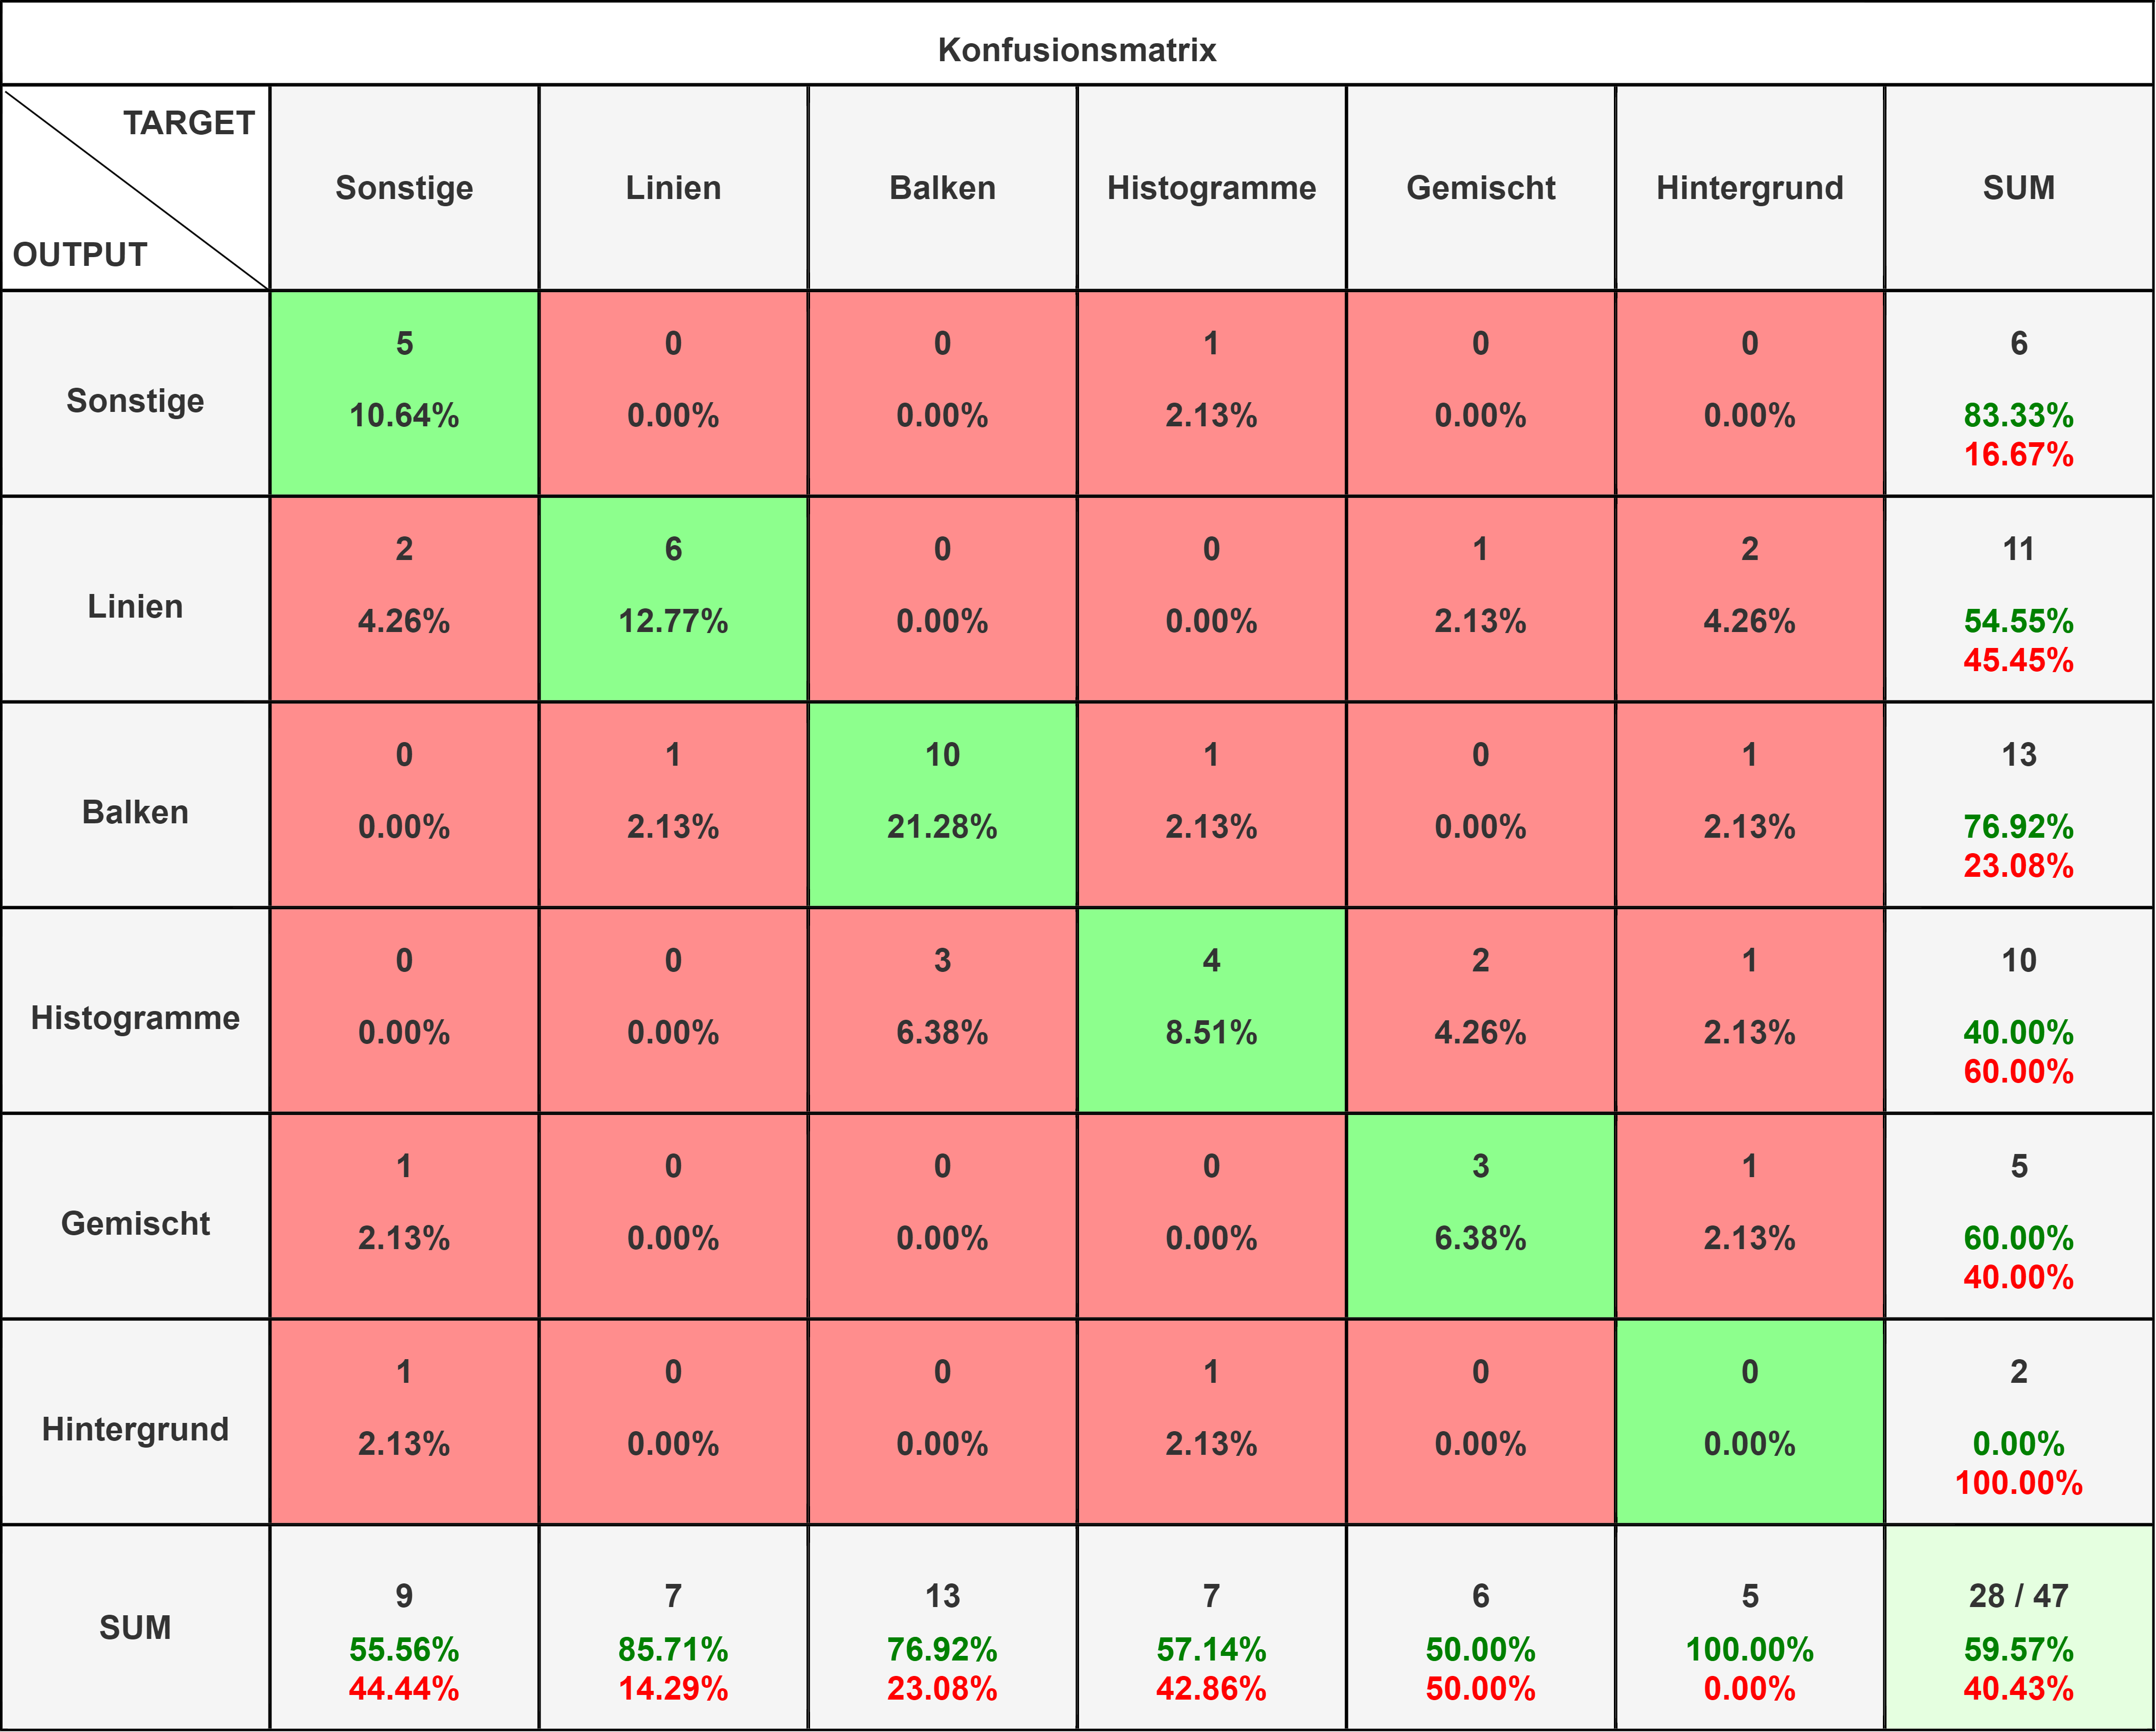
\includegraphics[width=1\textwidth]{Experimente/img/detect/1_val@0.404_200_histo/konfusionsmatrix.png}
    \caption{\hbadness=10000 x}
    \label{fig:extraction_output}
\end{figure}

\begin{table}[H]
    \centering
    \begin{tabular}{|l|c|c|c|}
        \hline
        \rowcolor[HTML]{EFEFEF}
                      & Precision & Recall    & F1-Score  \\ \hline
        Sonstige      & 83.33\%   & 55.56\%   & 66.67\%   \\ \hline
        Linien        & 54.55\%   & 85.71\%   & 66.67\%   \\ \hline
        Balken        & 76.92\%   & 76.92\%   & 76.92\%   \\ \hline
        Histogramme   & 60.00\%   & 57.14\%   & 47.06\%   \\ \hline
        Gemischt      & 40.00\%   & 50.00\%   & 54.55\%   \\ \hline
        \textbf{Alle} & \textbf{} & \textbf{} & \textbf{} \\ \hline
    \end{tabular}
    \caption{x}
\end{table}


\begin{figure}[H]
    \centering
    \captionsetup{width=1\linewidth}
    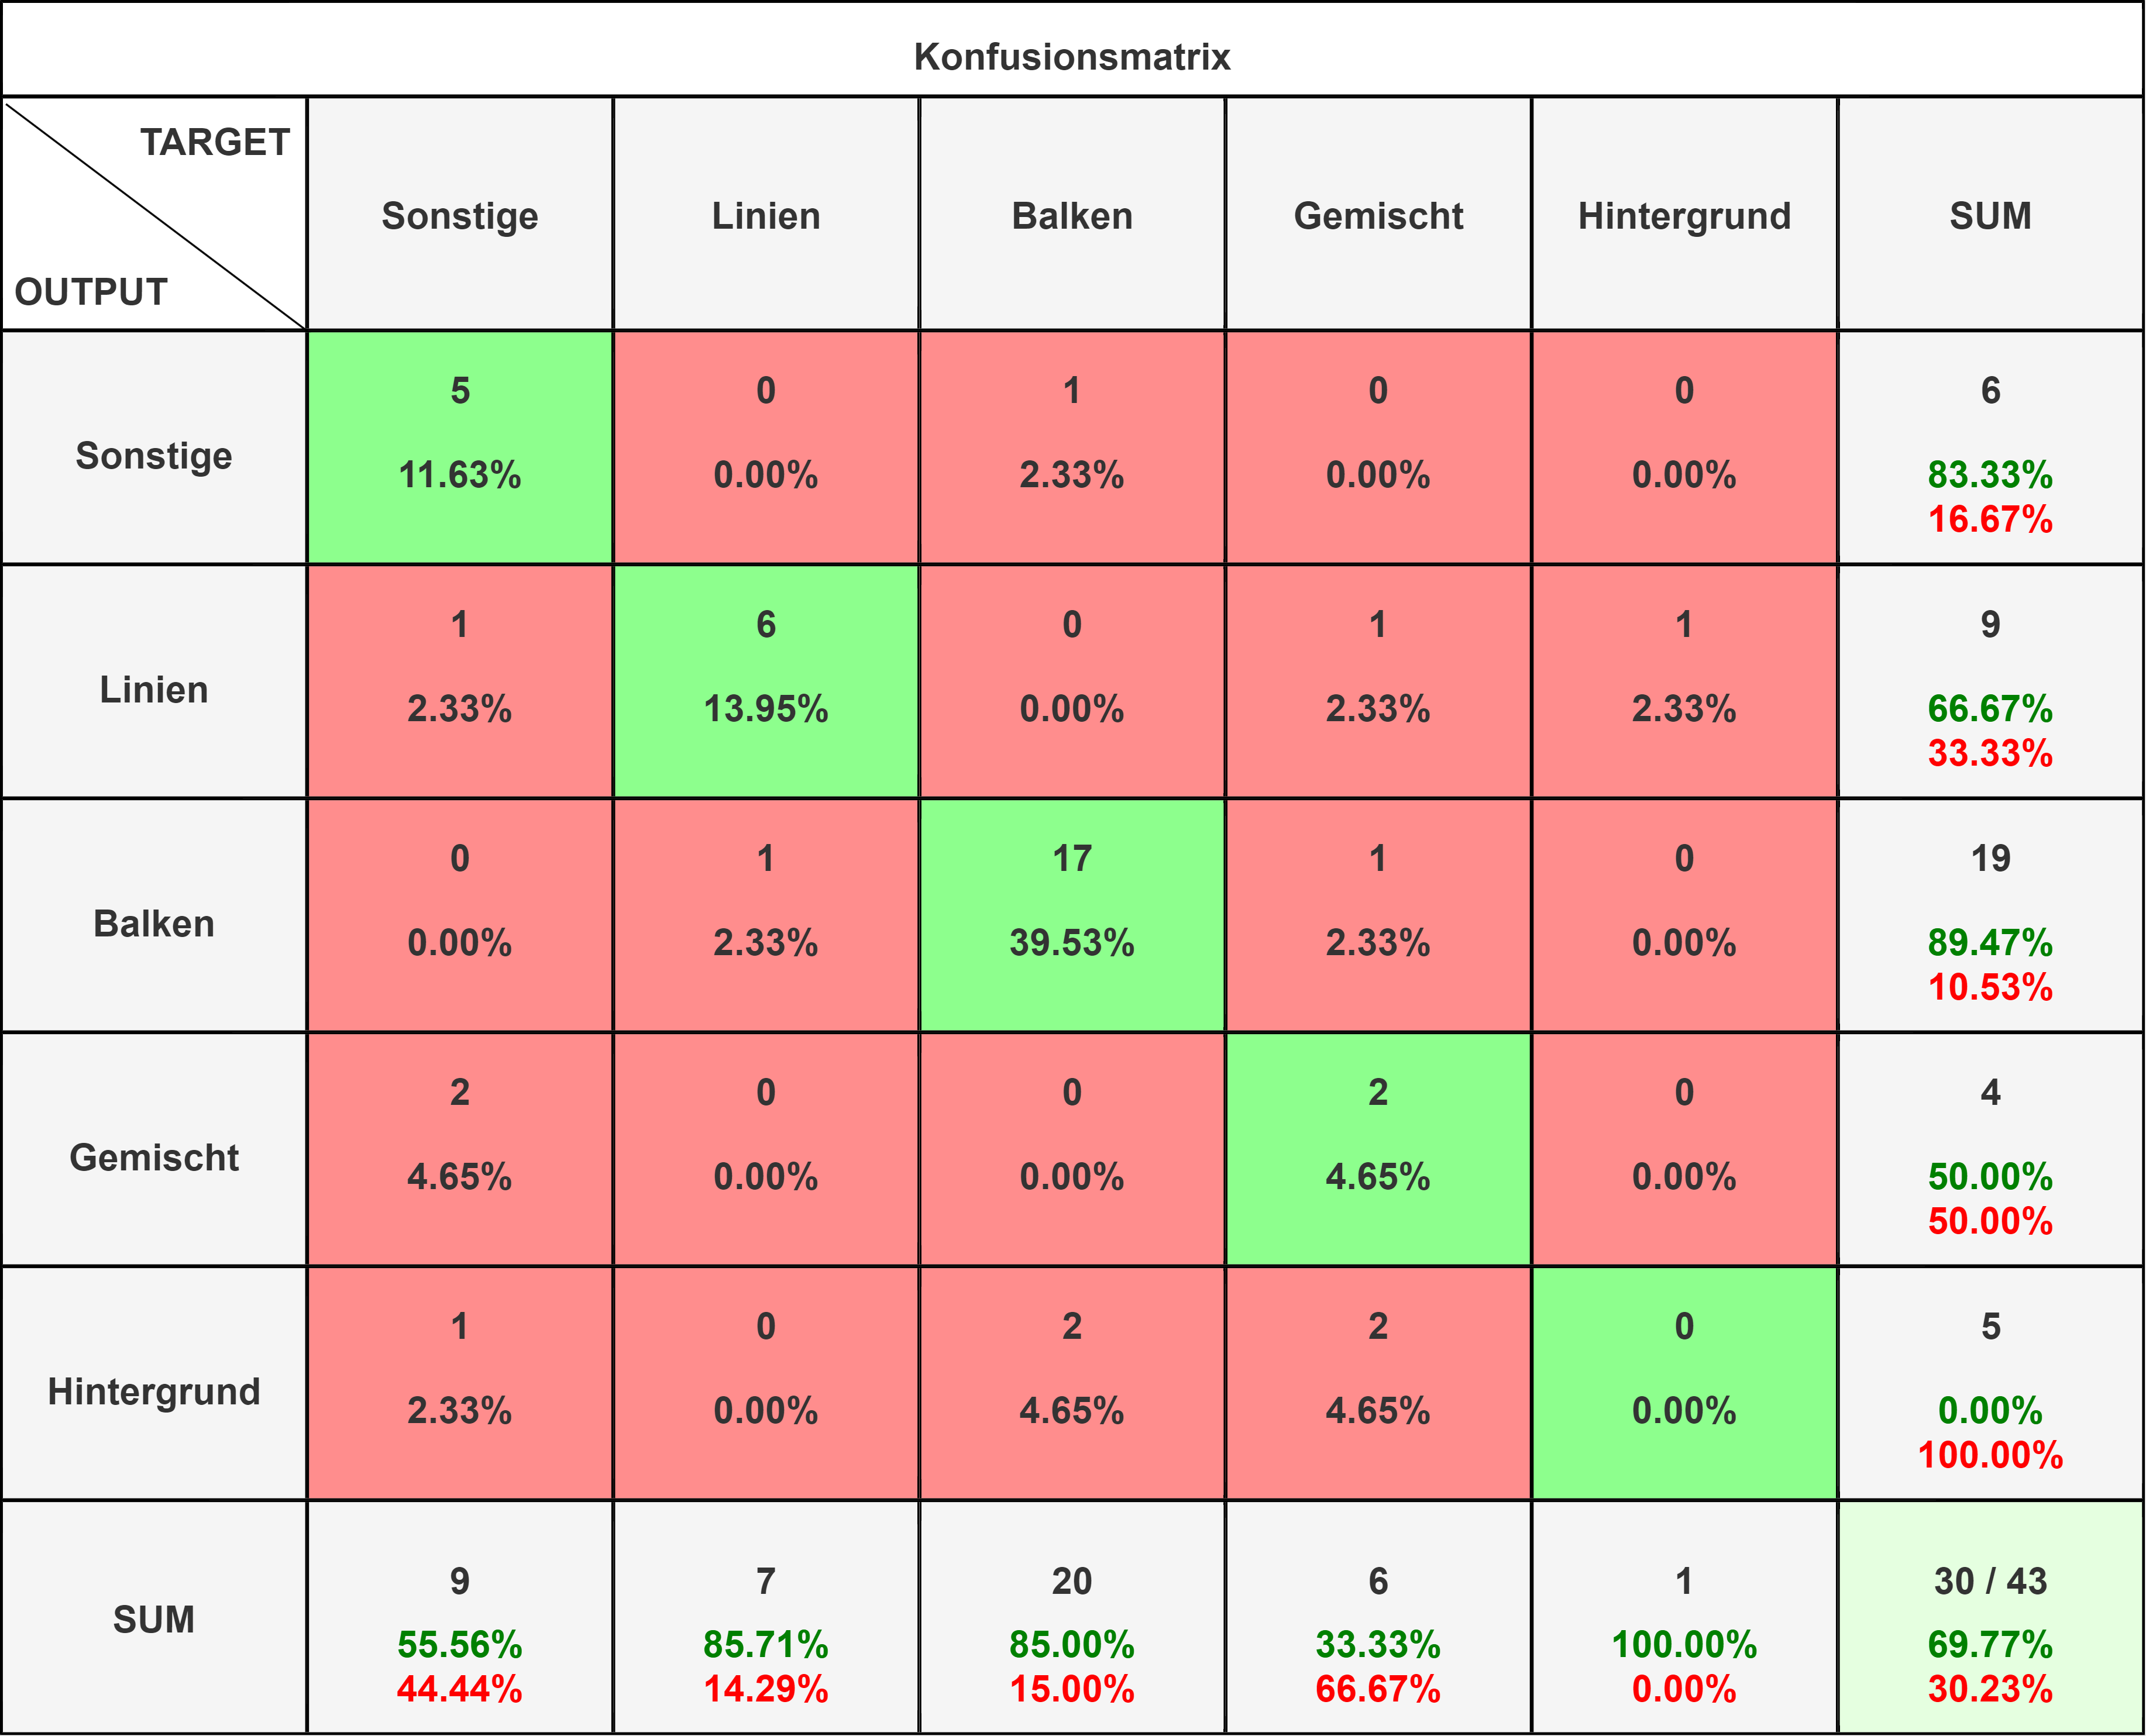
\includegraphics[width=1\textwidth]{Experimente/img/detect/2_val@0.511_200_nohisto/konfusionsmatrix.png}
    \caption{\hbadness=10000 x}
    \label{fig:extraction_output}
\end{figure}

\begin{table}[H]
    \centering
    \begin{tabular}{|l|c|c|c|}
        \hline
        \rowcolor[HTML]{EFEFEF}
                      & Precision & Recall    & F1-Score  \\ \hline
        Sonstige      & 83.33\%   & 55.56\%   & 66.67\%   \\ \hline
        Linien        & 66.67\%   & 85.71\%   & 75.00\%   \\ \hline
        Balken        & 89.47\%   & 85.00\%   & 87.18\%   \\ \hline
        Gemischt      & 50.00\%   & 33.33\%   & 40.00\%   \\ \hline
        \textbf{Alle} & \textbf{} & \textbf{} & \textbf{} \\ \hline
    \end{tabular}
    \caption{x}
\end{table}


\begin{figure}[H]
    \centering
    \captionsetup{width=1\linewidth}
    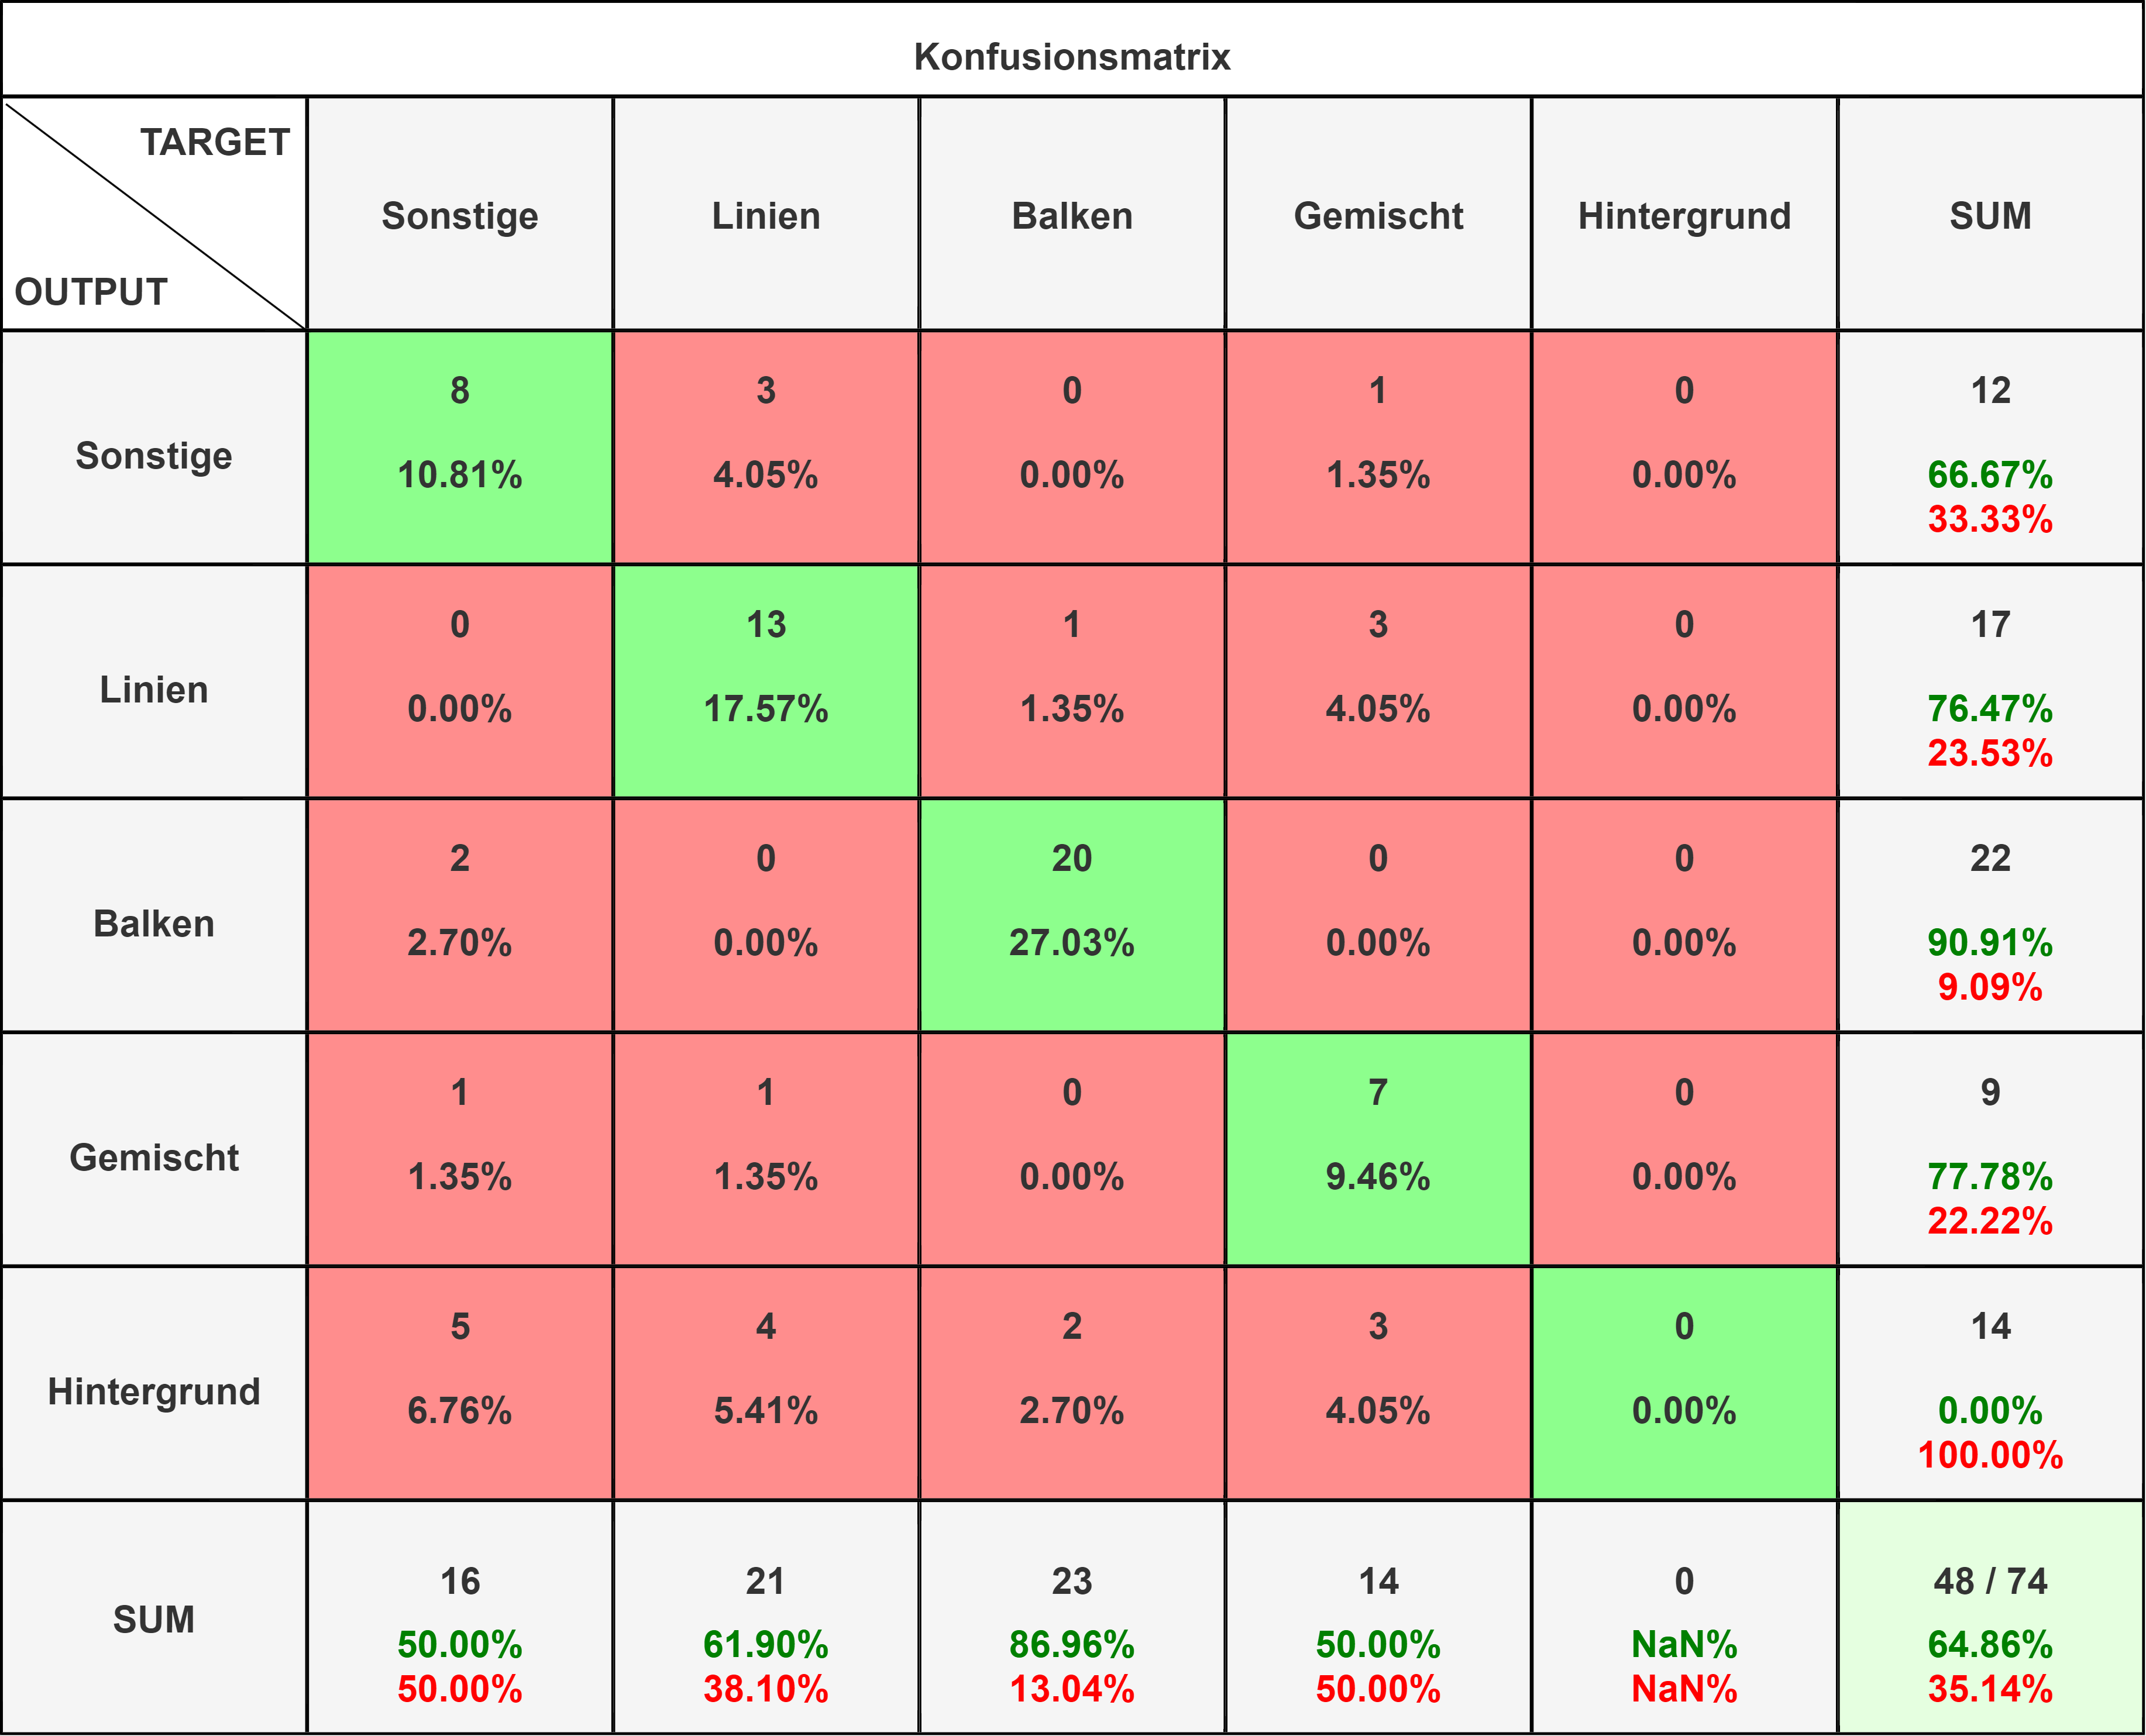
\includegraphics[width=1\textwidth]{Experimente/img/detect/3_val@0.653_nohisto/konfusionsmatrix.png}
    \caption{\hbadness=10000 x}
    \label{fig:extraction_output}
\end{figure}

\begin{table}[H]
    \centering
    \begin{tabular}{|l|c|c|c|}
        \hline
        \rowcolor[HTML]{EFEFEF}
                      & Precision & Recall    & F1-Score  \\ \hline
        Sonstige      & 66.67\%   & 50.00\%   & 57.14\%   \\ \hline
        Linien        & 76.47\%   & 61.90\%   & 68.42\%   \\ \hline
        Balken        & 90.91\%   & 86.96\%   & 88.89\%   \\ \hline
        Gemischt      & 77.78\%   & 50.00\%   & 60.87\%   \\ \hline
        \textbf{Alle} & \textbf{} & \textbf{} & \textbf{} \\ \hline
    \end{tabular}
    \caption{x}
\end{table}






\subsection{Feintraining auf historische Wirtschaftsscans}
\begin{figure}[H]
    \centering
    \captionsetup{width=1\linewidth}
    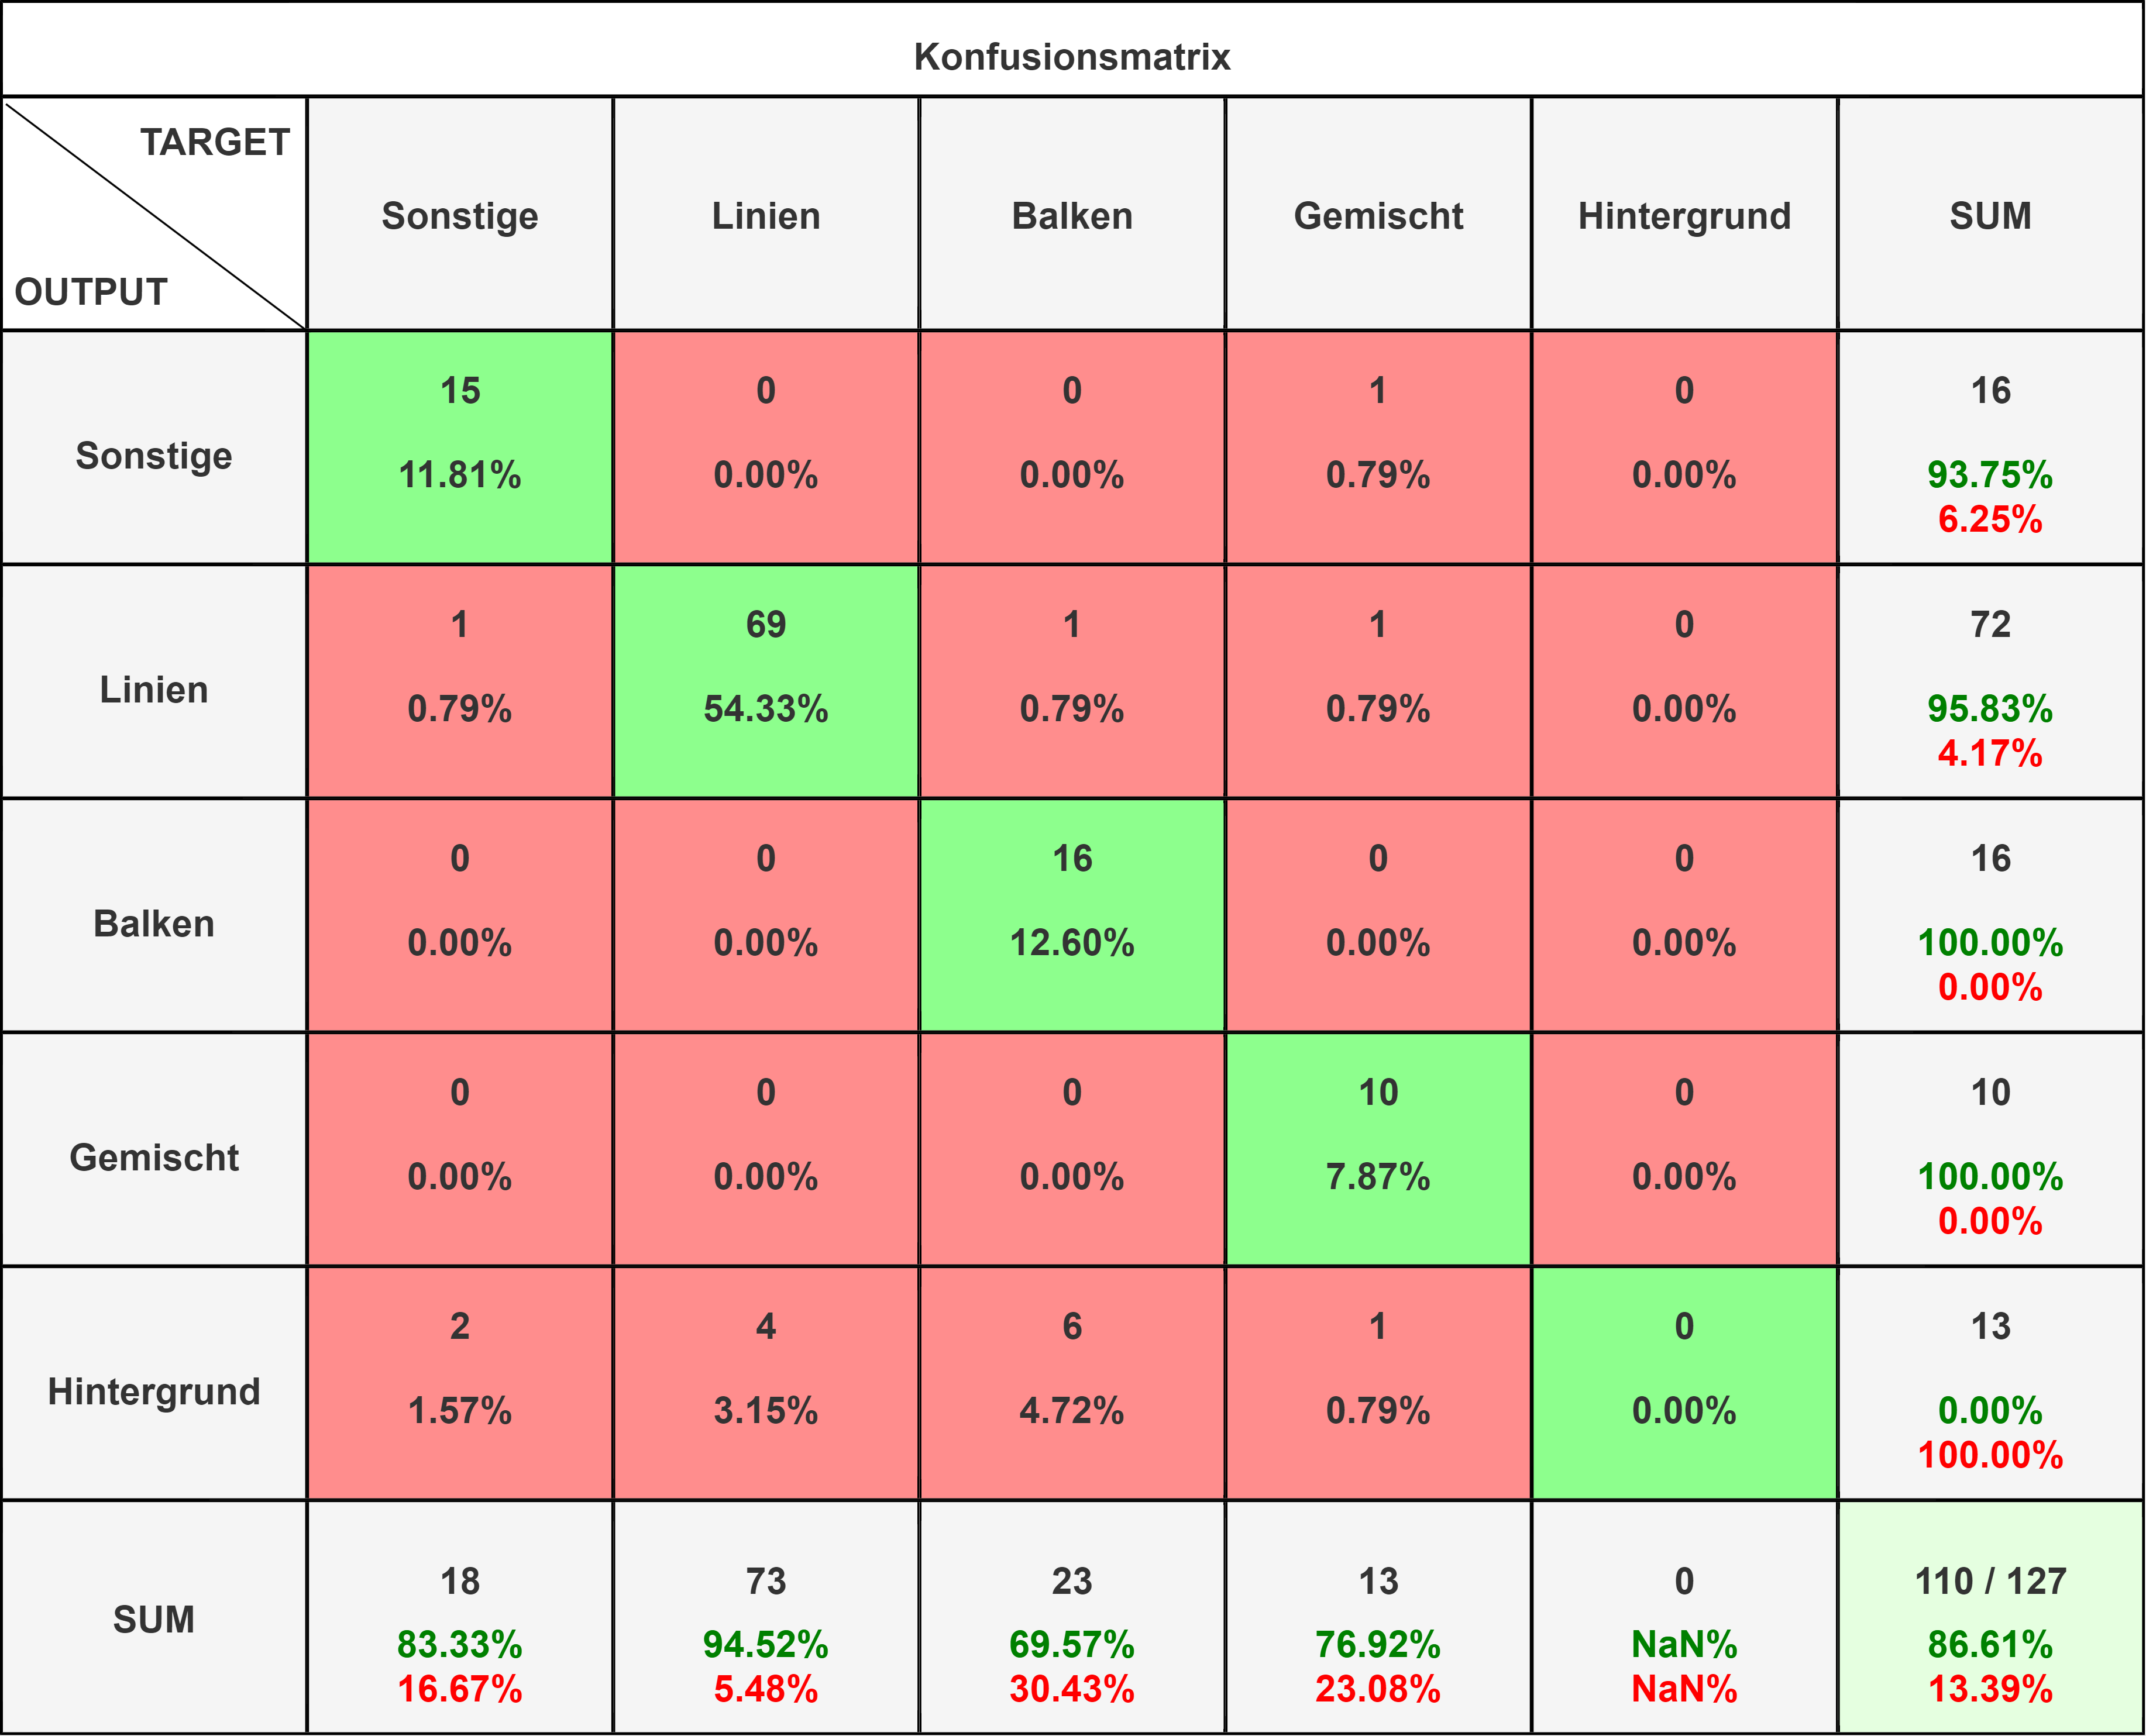
\includegraphics[width=1\textwidth]{Experimente/img/detect/val@0.891 20240612-093743_double/konfusionsmatrix.png}
    \caption{\hbadness=10000 x}
    \label{fig:extraction_output}
\end{figure}

\begin{table}[H]
    \centering
    \begin{tabular}{|l|c|c|c|}
        \hline
        \rowcolor[HTML]{EFEFEF}
                      & Precision      & Recall         & F1-Score       \\ \hline
        Sonstige      & 93.75\%        & 83.33\%        & 88.24\%        \\ \hline
        Linien        & 95.83\%        & 94.52\%        & 95.17\%        \\ \hline
        Balken        & 100.0\%        & 69.57\%        & 82.05\%        \\ \hline
        Gemischt      & 100.0\%        & 76.92\%        & 86.96\%        \\ \hline
        \textbf{Alle} & \textbf{0.974} & \textbf{0.811} & \textbf{0.881} \\ \hline
    \end{tabular}
    \caption{x}
\end{table}


\section{Liniendiagrammsklassifizierung}
\begin{figure}[H]
    \centering
    \captionsetup{width=1\linewidth}
    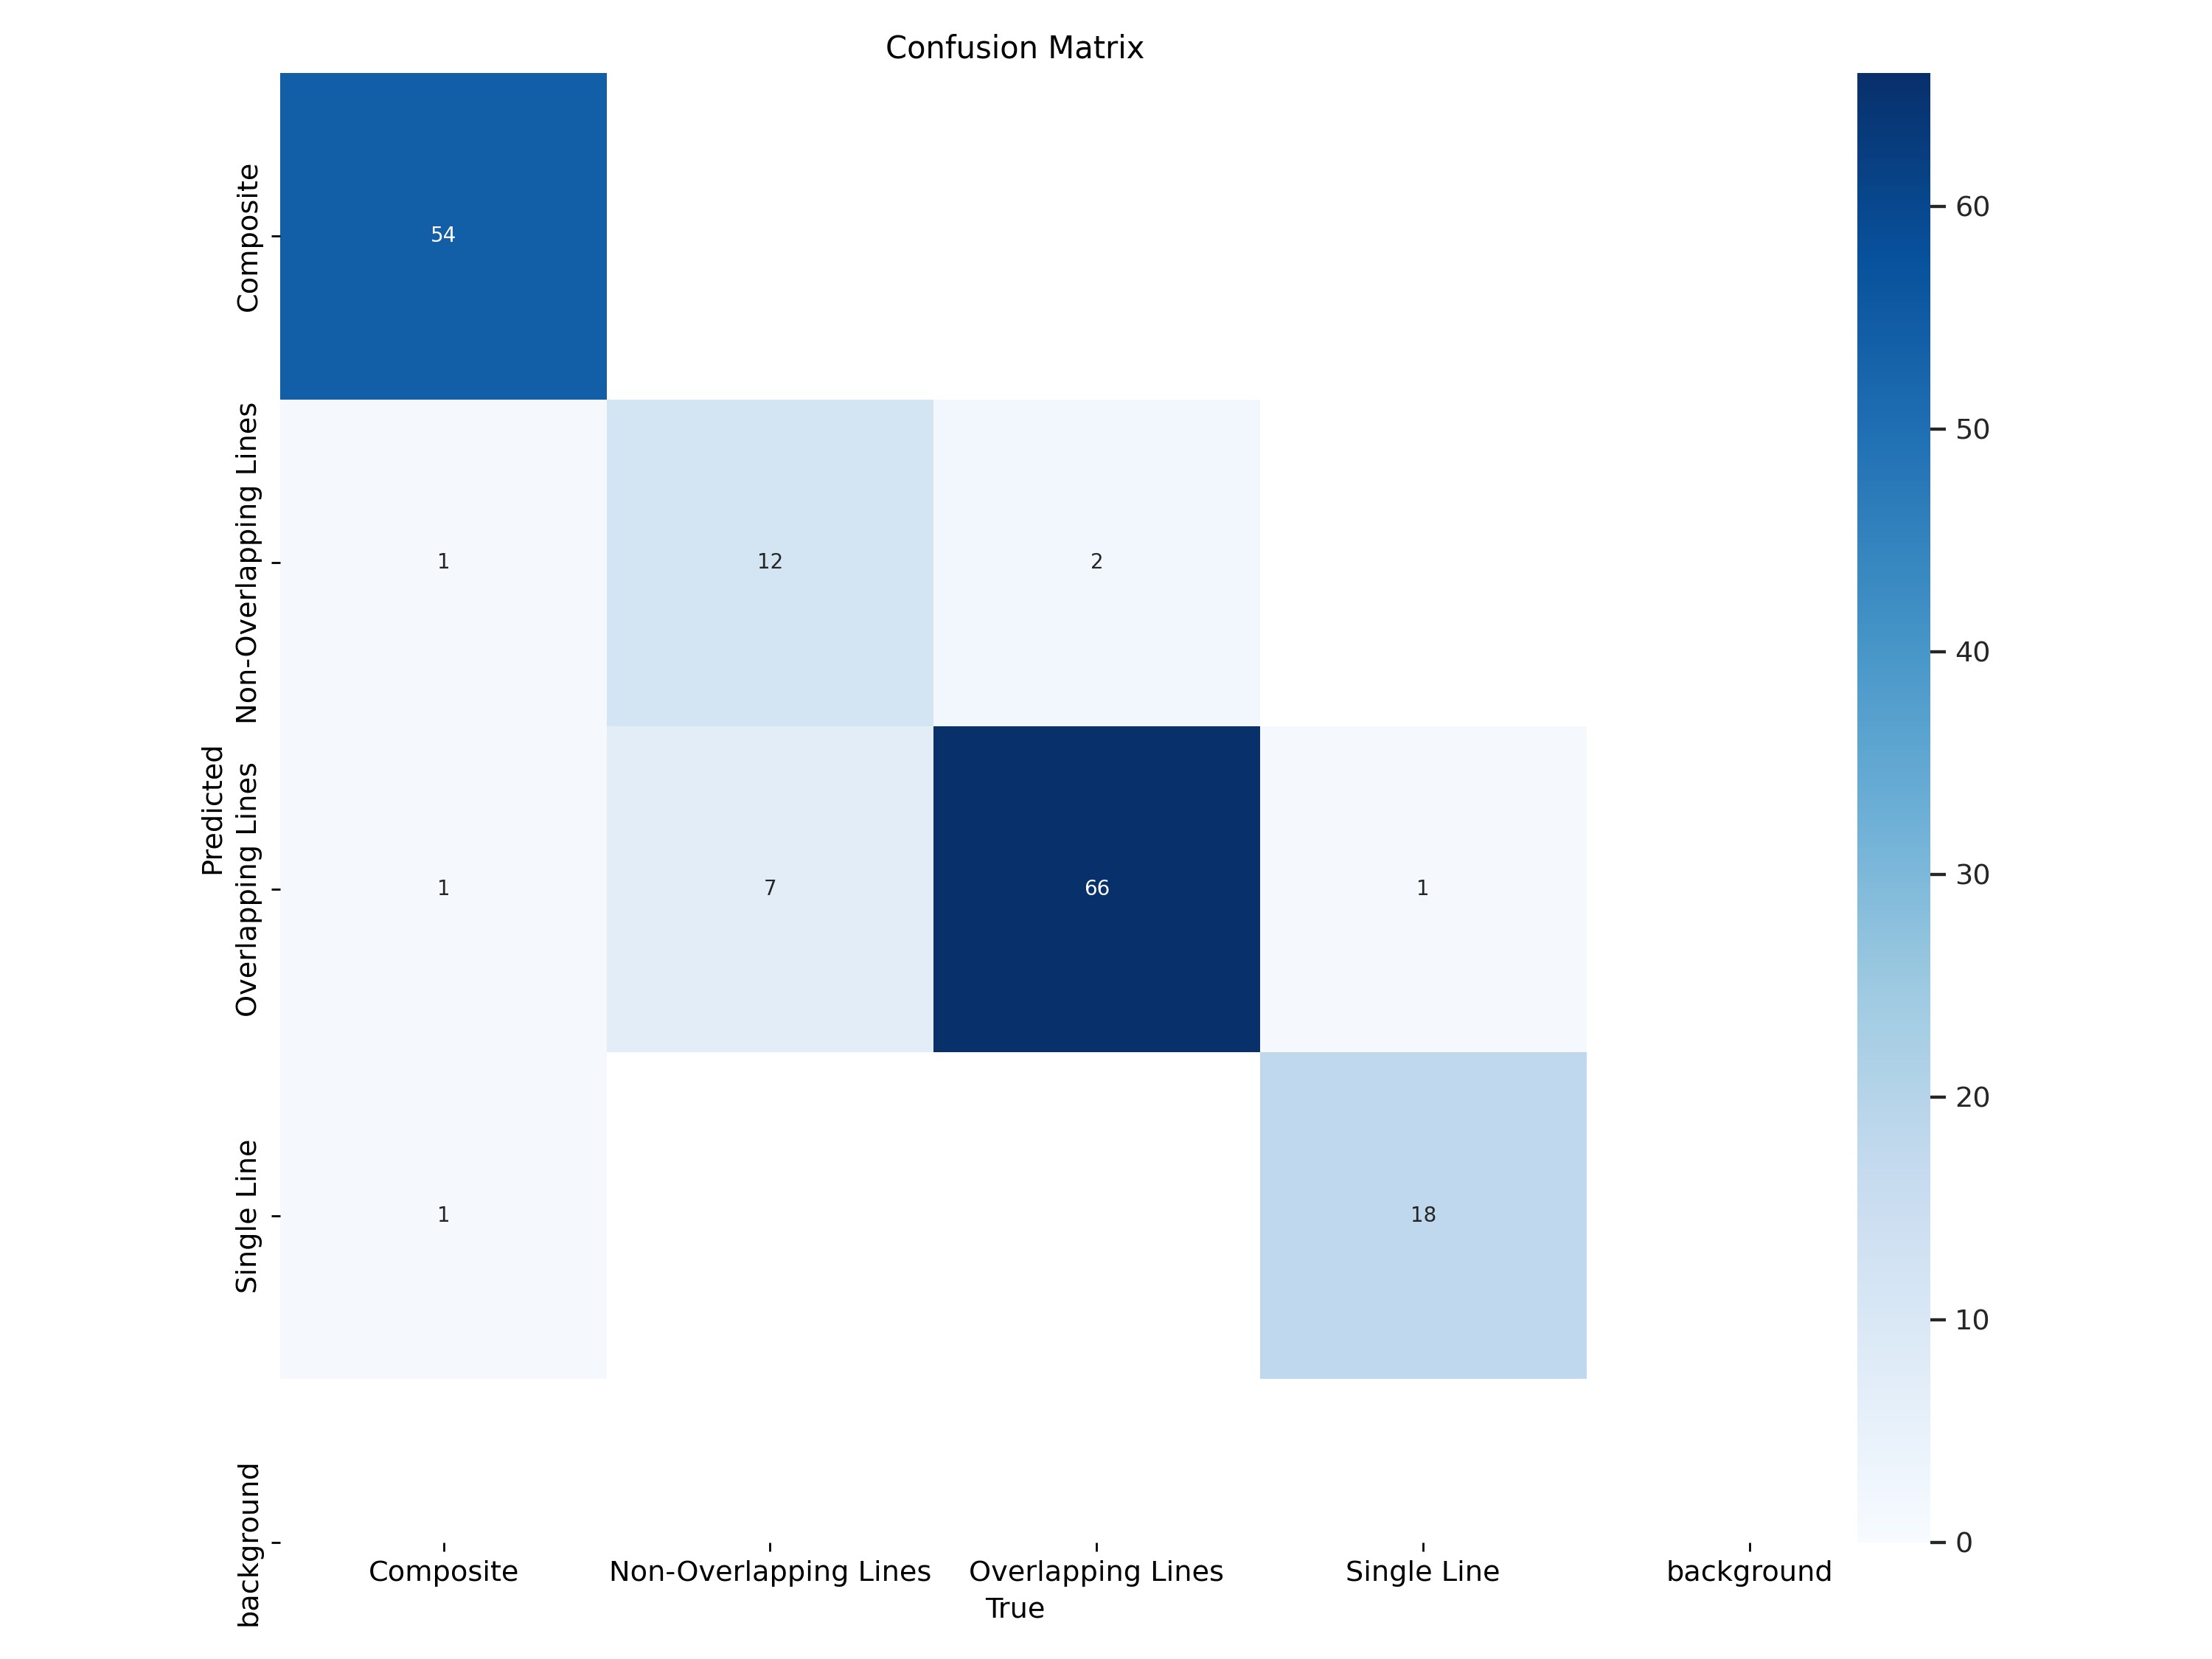
\includegraphics[width=1\textwidth]{Experimente/img/classify/val_v1/confusion_matrix.png}
    \caption{\hbadness=10000 x}
    \label{fig:extraction_output}
\end{figure}
\begin{figure}[H]
    \centering
    \captionsetup{width=1\linewidth}
    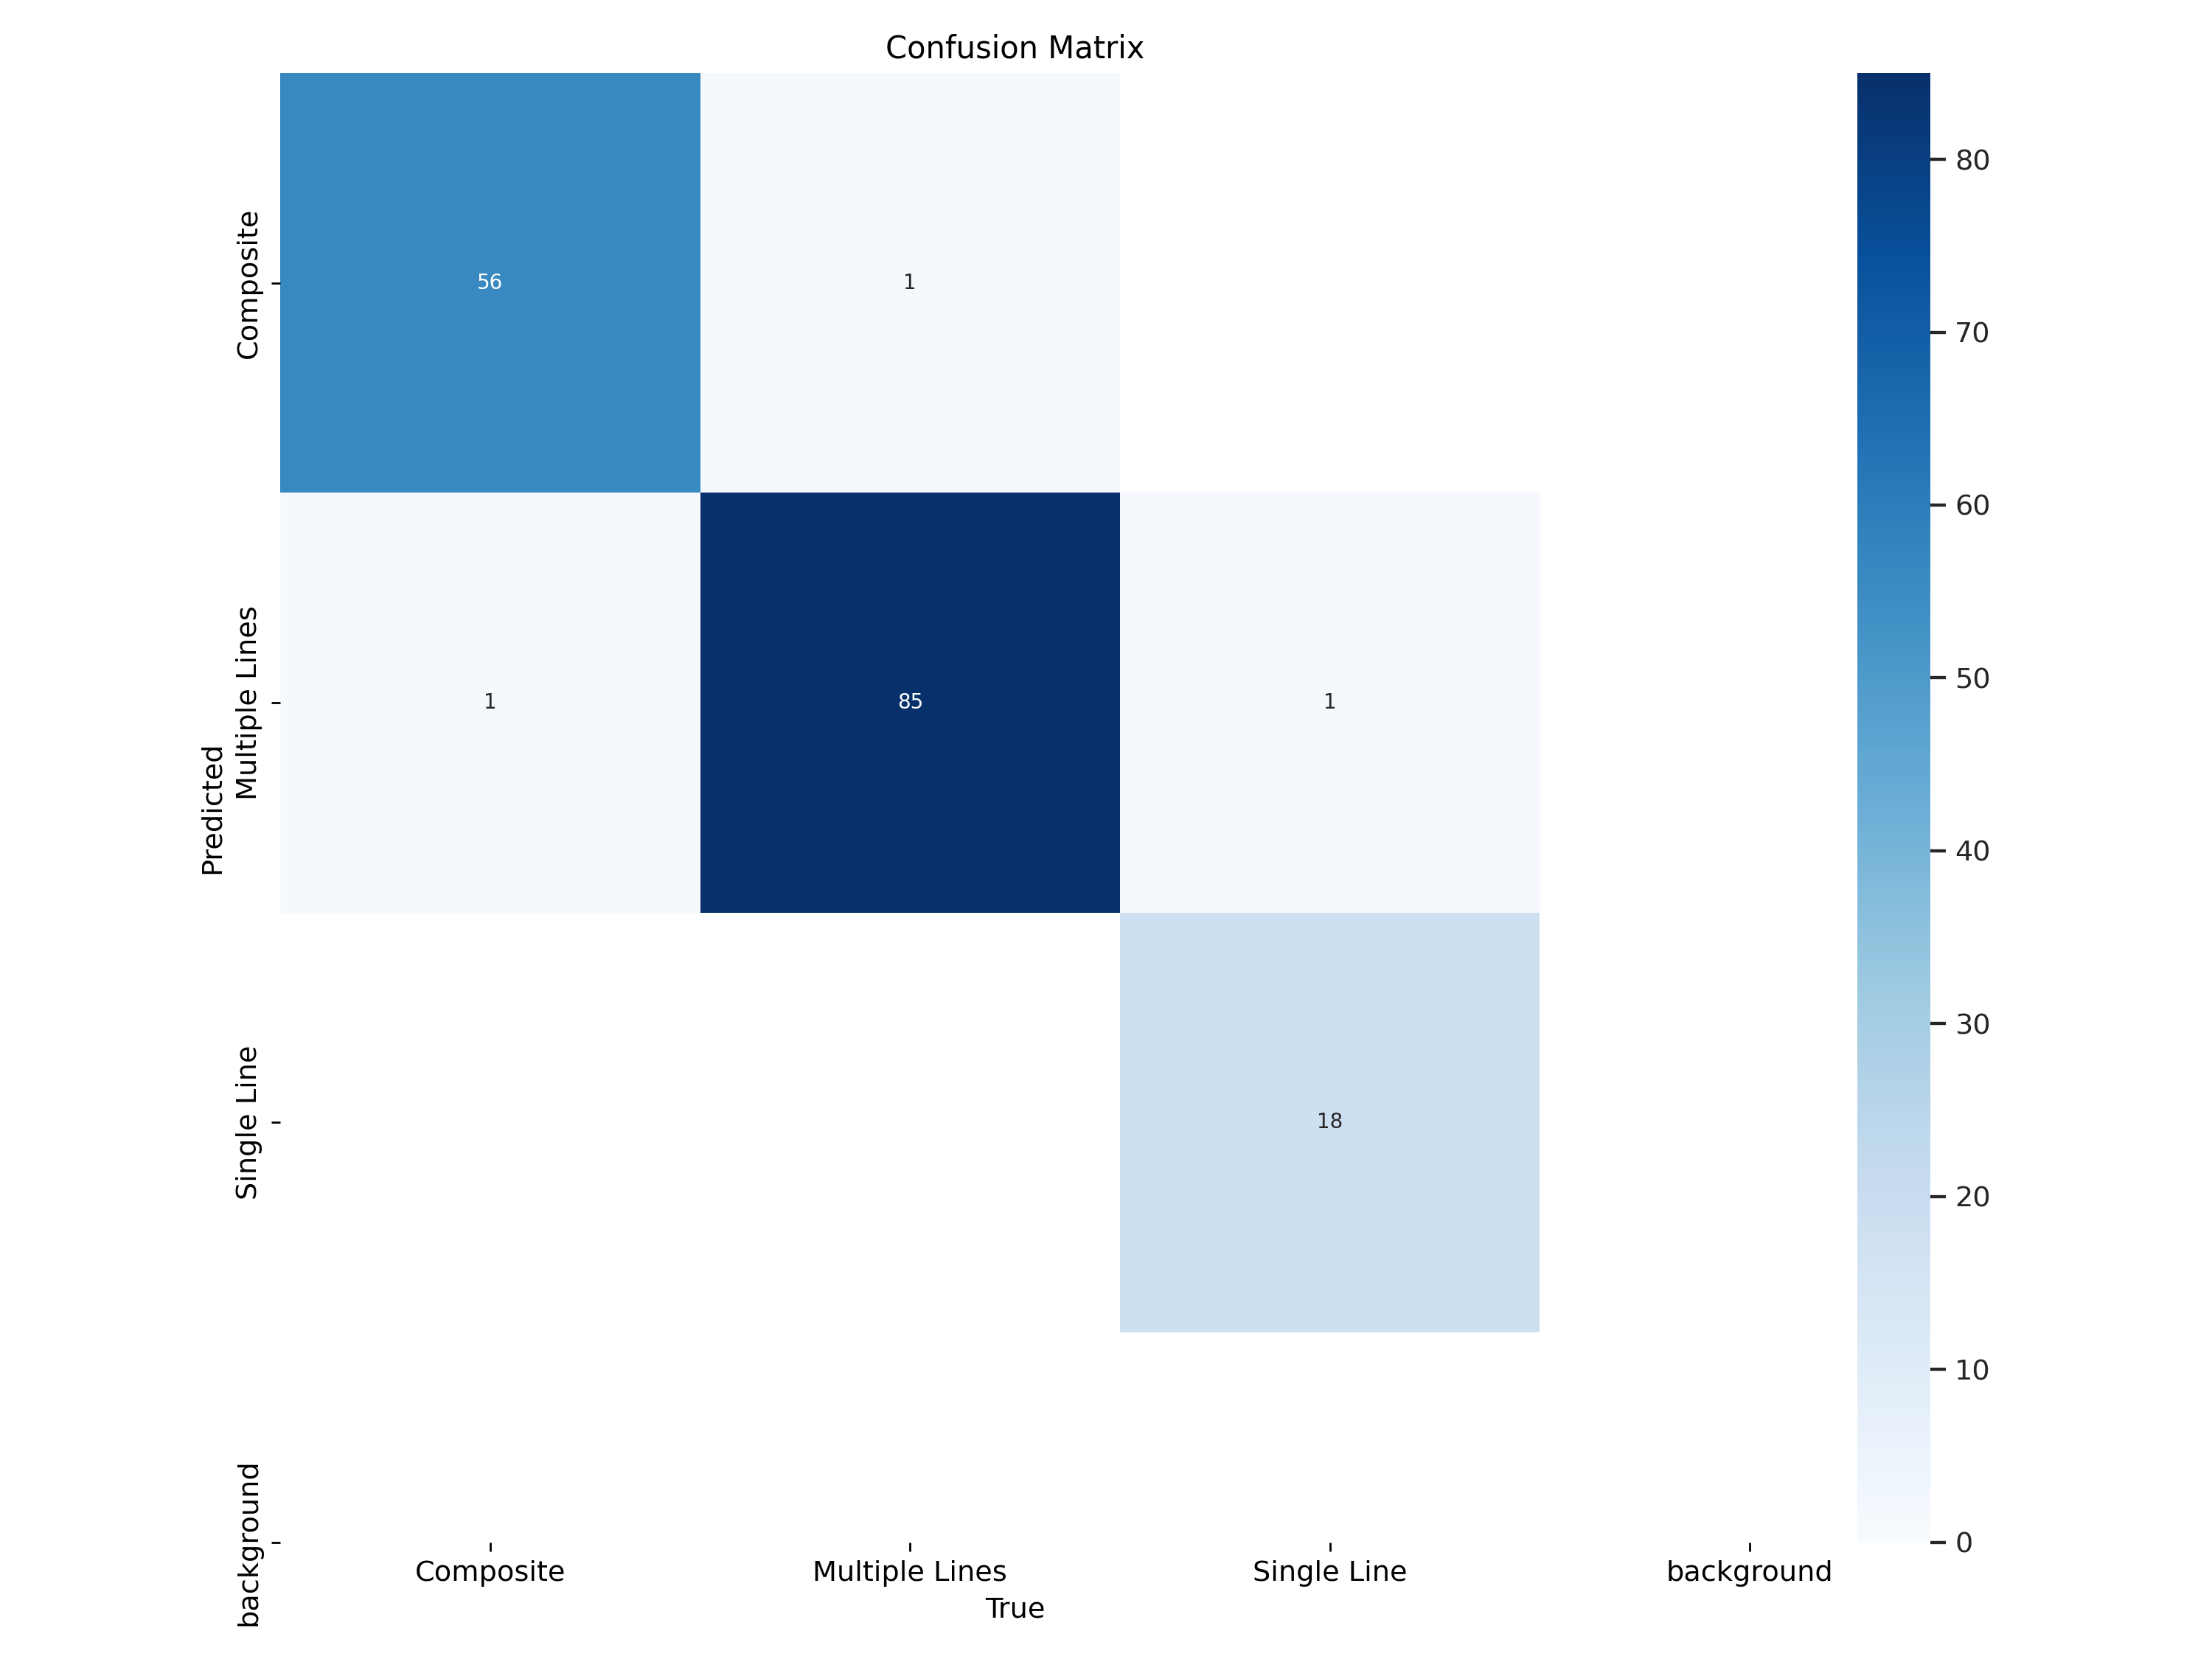
\includegraphics[width=1\textwidth]{Experimente/img/classify/val_v2/confusion_matrix.png}
    \caption{\hbadness=10000 x}
    \label{fig:extraction_output}
\end{figure}

\section{Segmentation}
\subsection{Instanzsegmentation durch Ultralytics YOLO}
\subsection{Semantische Segmentation durch das U-Net}

\section{Diagrammsauswertung}
\subsection{Achsenerkennung durch OCR}
\subsection{Numerische Tabellenformextraktion}


Die verwendeten Metriken bei der Objekterkennung fassen sich aus Präzision (precision), Erinnerung (recall), mAP50 und mAP50-95 zusammen. Zum Berechnen dieser wird das Aufkommen der Richtig Positiven (TP), Falsch Positiven (FP) und Falsch Negativen (FN) Vorhersagen (predictions) des Modells benutzt. Die Kategorie TP zeigt vom Modell richtig erkannte Objekte, welche tatsächlich vorhanden sind, FP bestimmt die falsche Erkennung des Modells von Objekten die in Wirklichkeit nicht vorhanden sind und FN gibt Auskunft über Objekte die in der Realität vorhanden sind, das Modell sie allerdings nicht erkannt hat.

\[Precision = \frac{TP}{TP + FP}\]

Precision misst den Anteil der korrekten positiven Vorhersagen an allen positiven Vorhersagen des Modells. Sie zeigt, wie genau das Modell bei der Erkennung von Objekten ist und wie gut es falsche positive Ergebnisse vermeidet. Ein hoher Precision-Wert bedeutet, dass wenn das Modell ein Objekt erkennt, es mit hoher Wahrscheinlichkeit tatsächlich vorhanden ist.

\[Recall = \frac{TP}{TP + FN}\]

Recall misst den Anteil der korrekt erkannten positiven Instanzen an allen tatsächlichen positiven Instanzen. Es zeigt, wie gut das Modell alle vorhandenen Objekte einer Klasse findet. Ein hoher Recall-Wert bedeutet, dass das Modell die meisten der tatsächlich vorhandenen Objekte erkennt.

\[mAP50 = \frac{1}{n} \sum_{i=1}^{n} AP_i\]
wobei $n$ die Anzahl der Klassen ist und $AP_i$ die durchschnittliche Präzision für die i-te Klasse bei IoU=0.5.

mAP50 (mittlere durchschnittliche Präzision bei IoU=0.5) misst die die Genauigkeit des Modells über alle Klassen hinweg. Dabei wird ein Intersection over Union (IoU) Schwellenwert von 0,5 verwendet. Eine Erkennung gilt als korrekt (TP), wenn die IoU zwischen der vorhergesagten und der tatsächlichen Bounding Box größer als 0,5 ist. Ein hoher mAP50-Wert zeigt, dass das Modell einfache Objekte verschiedener Klassen zuverlässig erkennt und lokalisiert.

\[\mathit{mAP50\mbox{-}95} = \frac{1}{10} \sum_{t=0.5}^{0.95} mAP_t\]
wobei $t$ die IoU-Schwellenwerte von 0.5 bis 0.95 in Schritten von 0.05 durchläuft.
\hbadness=10000\\\\
mAP50-95 (mittlere durchschnittliche Präzision bei IoU=0.5:0.95) ist misst die Leistung des Modells über verschiedene IoU-Schwellenwerte. Sie berechnet den Durchschnitt der mAP-Werte für alle IoU-Schwellenwerte von 0,5 bis 0,95 in Schritten von 0,05. Dies gibt einen robusteren Überblick über die Modellleistung, da es verschiedene Grade der Überlappungsgenauigkeit berücksichtigt. Ein hoher mAP50-95-Wert zeigt, dass das Modell sowohl bei einfachen als auch bei schwereren Eingaben zuverlässige Vorhersagen trifft.
\hbadness=10000\\\\\\
Im Kapitel "Experimente" Ihrer Bachelorarbeit sollten Sie die durchgeführten Versuche, deren Ergebnisse und Ihre Analyse darlegen. Hier ist eine Übersicht der wichtigsten Punkte, die in diesem Kapitel enthalten sein sollten:

Versuchsaufbau:

Beschreibung der verwendeten Datensätze (Trainings-, Validierungs- und Testdaten)
Erklärung der Evaluierungsmetriken (z.B. mAP für YOLO, IoU für U-Net)
Definition der Baseline oder Vergleichsmodelle


Durchgeführte Experimente:

Detaillierte Beschreibung jedes einzelnen Experiments
Begründung für die Wahl der Experimente
Variationen in Hyperparametern, Modellarchitekturen oder Trainingsmethoden


Ergebnisse:

Präsentation der quantitativen Ergebnisse (in Tabellen oder Grafiken)
Qualitative Ergebnisse (z.B. Beispielbilder von Vorhersagen)
Vergleich der Leistung von YOLO und U-Net für Ihre spezifische Aufgabe


Analyse:

Interpretation der Ergebnisse
Diskussion von Stärken und Schwächen der Modelle
Vergleich mit dem aktuellen Stand der Technik oder anderen relevanten Arbeiten


Ablationstudie:

Untersuchung des Einflusses verschiedener Komponenten oder Hyperparameter auf die Modellleistung


Fehleranalyse:

Identifikation von häufigen Fehlertypen
Diskussion möglicher Gründe für diese Fehler


Laufzeitanalyse und Ressourcenverbrauch:

Vergleich der Inferenzzeiten von YOLO und U-Net
Analyse des Speicher- und Rechenbedarfs


Diskussion der Limitationen:

Grenzen der durchgeführten Experimente
Mögliche Verzerrungen in den Daten oder der Evaluation


Zukünftige Arbeiten:

Vorschläge für weitere Experimente oder Verbesserungen basierend auf Ihren Ergebnissen



Dieses Kapitel sollte eine objektive Darstellung Ihrer experimentellen Arbeit sein, die es dem Leser ermöglicht, die Leistung und Eignung von YOLO und U-Net für Ihre spezifische Anwendung zu verstehen und zu bewerten.